% Small intro, re-explain that finding thread/core pairing is complicated and thus ML is a good idea.
As seen in the previous section, selecting the right number of threads and a good combination of cores is difficult.
This difficulty arises from trying to balance between exploiting ILP by fusing a large amount of cores and TLP by generating more threads.
As the design space is large, it is important to automate the decision making to alleviate the task of getting the best performance out of the streaming application at hand.

The problem of automating this decision can be decomposed into two stages; first, determining the right number of threads and second, selecting a good core composition.
In this section, two machine-learning models that predict the best thread partitioning and core composition to maximize performance are presented.

\subsection{Synthetic Benchmark Generation}

One of the difficulties of building a machine learning based model for StreamIt is the lack of benchmarks available~\cite{wang2013partitionstreamit}.
Whilst there exists at least 30 realistic applications for StreamIt~\cite{theis2010empericalcharstreamit} this is simply not enough to create a large enough data set.
To overcome this problem generating synthetic benchmarks can be a solution~\cite{cumminsopencl2017}.
Thus synthetic StreamIt benchmarks are generated and statistics are gathered from them in a similar style as in~\cite{wang2013partitionstreamit}.
To ensure that the synthetic benchmarks are representative of realistic benchmarks they are created using filters from a set of micro-kernels found in some StreamIt applications.
30 different possible filters with different incoming and outgoing rates and different inputs and outputs types are used to increase the variety of the dataset.
To ensure that the synthetic benchmarks are similar to real benchmarks, the total number of filters and split joins are within the average of the realistic benchmarks.

For each generated application, 15 different threaded versions are generated.
Each of these versions is ran using a single core per thread and the cycle count is recorded.
This was repeated for 1000 unique randomly generated applications and record the best number of threads each time.

Once the benchmarks have been generated, the next step consists of gathering features for each applications.
In order to build the two machine learning models an initial set of over 50 features are extracted from StreamIt programs.
These features are extracted using pre-existing analytical tools within StreamIt and some counters added specifically for this chapter.
As 50 features may not necessarily contain any valuable information, the features selected for the models are determined through correlation analysis.
%In this section, when discussing correlation we specifically look at which variables correlate with the optimal number of threads.

\subsection{Correlation Analysis and kNN model}
In this section, variables which correlate with the optimal number of threads are explored.
These features are used by the model to make a prediction about the number of threads to use.
Figure~\ref{fig:corr} shows the 10 variables that correlate the most with determining the optimal thread number.
In StreamIt the term \textit{multiplicity} defines the number of times a filter will have to execute in a time slice when the graph is in a steady state~\cite{gordon2002streamcomp}.

\begin{figure}
  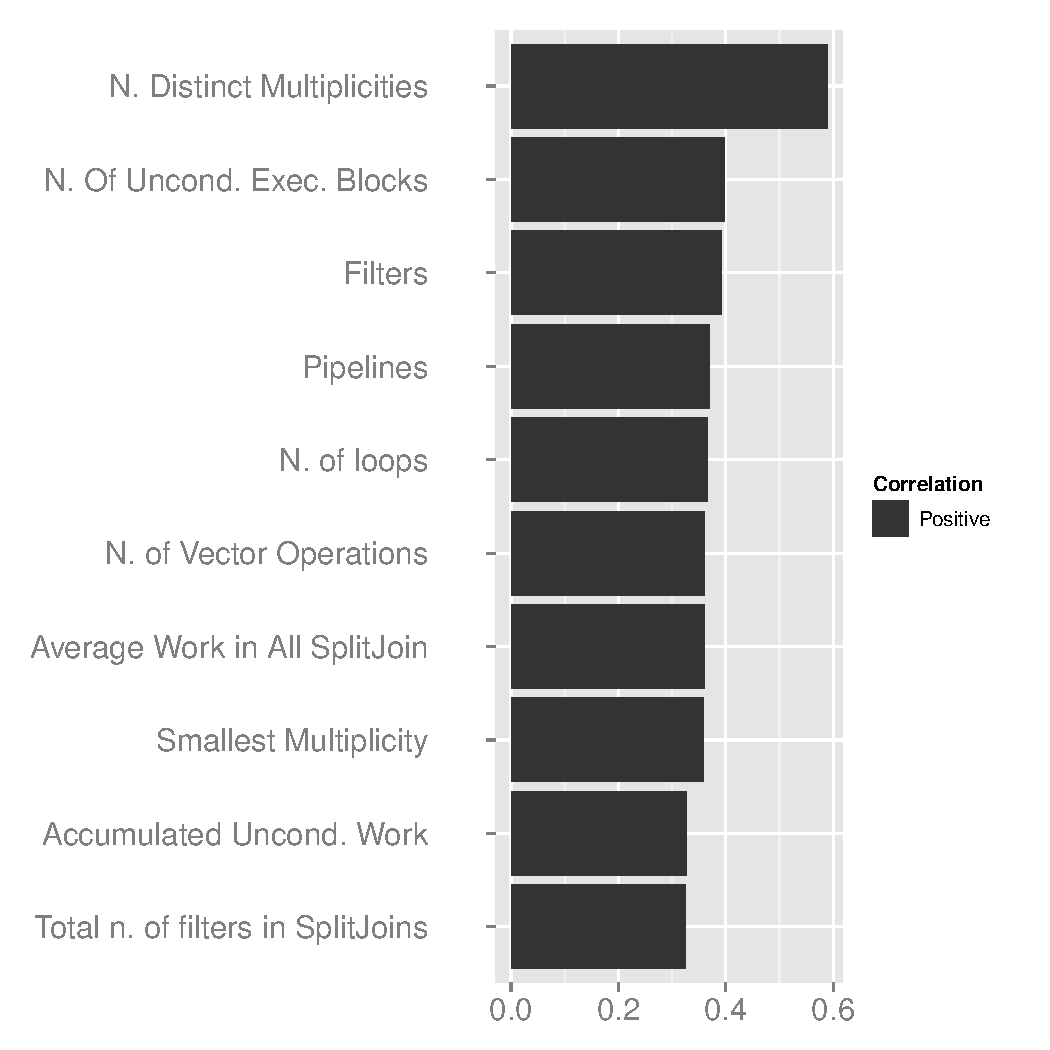
\includegraphics[width=1\textwidth]{streamit-paper/graphics/corrGraph.pdf}
  \caption{The ten highest correlating features with the best number of threads for 1000 synthetic benchmarks.}\label{fig:corr}
\end{figure}
 
The 10 features can be described as followed:
\begin{itemize}
\item Number of Distinct Multiplicities: the variety of different execution rates of filters per time slice.
\vspace{-1em}
\item Number of unconditionally executed blocks: amount of operations in a filter that always execute.
\vspace{-1em}
\item Filters: number of filters found in the benchmark.
\vspace{-1em}
\item Pipelines: number of pipelines found in the benchmark.
\vspace{-1em}
\item Number of Loops: amount of loops present in the benchmark.
\vspace{-1em}
\item Number of Vector Operations: amount of potential vector operations found in the benchmark.
\vspace{-1em}
\item Average Work in all SplitJoins: average amount of operations per SplitJoin.
\vspace{-1em}
\item Smallest Multiplicity: The smallest execution rate of a single filter.
\vspace{-1em}
\item Accumulated Unconditional Work: Total number of operations in all filters which must be executed.
\vspace{-1em}
\item Total Number of filters in SplitJoins: Amount of filters that are found in SplitJoins.
\end{itemize}

According to Figure~\ref{fig:corr} the highest correlating value is Number of Distinct Multiplicitie found in the StreamIt application.
There are very little variables that highly correlate beyond Number of Distinct Multiplicities.
A high number of distinct multiplicities implies that the StreamIt application features an important amount of filters with different execution rates.
This means that certain filters may be local bottlenecks in a Pipeline for example.
Multithreading the pipelines with local bottlenecks will help alleviate the problem of multiple distinct multiplicities.
For example, the benchmark \bench{ChannelVocoder} only has 66\% of its filters sharing the same average multiplicity of 50~\cite{theis2010empericalcharstreamit}, with a minimum multiplicity of 1. 
The benchmark features a single SplitJoin yet when recalling section \ref{sec:streamit:dse}'s Figure~\ref{fig:overviewhist} \bench{ChannelVocoder}'s performance is greatly improved via multi-threading.
The number of threads also depends on certain structural features such as Pipelines, SplitJoins and number of Filters.
Yet, these variables seem to hold less influence on the number of threads a program needs than the different multiplicities found in the graph.
This is most certainly due to the fact that whilst SplitJoins make parallelizable areas more visible, the amount of work contained in each stream of the SplitJoin, especially when this size is small, may actually make parallelizing the program worse due to ratio of communication to computation.
It is also important to understand that a high number of Pipelines implies the use of SplitJoins.
This is due to the fact that a StreamIt application with no SplitJoins will feature only a singe Pipeline, thus a larger number of pipelines implies at least one SplitJoin.
This is why the number of SplitJoins is not present in the correlating features; because the number of Pipeline already correlates with this feature.\\

A k-Nearest Neighbor (kNN) model is deployed to determine the number of threads to use for an application.
Given a new application, the kNN classifier determines the $k$ closest generated applications.
The distance between the features is measured using the Euclidean for each application.
Once the set of $k$ nearest neighbors is identified, the model simply averages the best number of threads for each of the $k$ nearest neighbors to make a prediction.
The parameter $k$ was determined experimentally using only the generated benchmarks.
A value of $k=7$ was found to lead to the best performance.
The features chosen are the ten variables displayed in Figure~\ref{fig:corr}.

Cross validation is used to determine the efficiency of the model by observing how close a classification is to the measured best thread number.
Using cross validation the model generated in this chapter has a 33\% accuracy of getting the exact best thread number.
The accuracy increases to 57\% when allowing a prediction to be 1 thread away from the best and 67\% when 2 threads away.
On average, having a thread number that is +/- 1 away from the optimal thread count only incurrs a 12\% performance penalty.
For a distance of +/- 2 this increases to 19\%.
This penalty was measured by comparing the performances of the synethtic benchmarks using only multithreading.


